% !TEX root = Projektdokumentation.tex
\section{Beispiel 3}
\label{sec:beispiel3}

\subsection{Ausgangssituation} 
\label{sec:ausgangssituation3}
Wie in Abschnitt \ref{sec:voraussetzungen} beschrieben, liefert die Schulze Methode auch Ergebnisse, wenn Kandidaten gleich bewertet wurden oder nicht bewertet wurden. Nicht bewertete Kandidaten werden dabei behandelt, als wären sie alle vom Wähler auf dem letzten Platz gewählt worden, sodass jeder Kandidat, der vom Wähler bewertet wurde, den nicht bewerteten Kandidaten vorgezogen wird.

\begin{description}
\centering
\item[6 mal] $a \succ_{v} b \succ_{v} c \succ_{v}d$
\item[8 mal] $a \approx_{v} b \succ_{v} c \approx_{v}d$
\item[8 mal] $a \approx_{v} c \succ_{v} b \approx_{v}d$
\item[18 mal] $a \approx_{v} c \succ_{v} d \succ_{v}b$
\item[8 mal] $a \approx_{v} c \approx_{v} d \succ_{v}d$
\item[40 mal] $b \succ_{v} a \approx_{v} c \approx_{v}d$
\item[4 mal] $c \succ_{v} b \succ_{v} d \succ_{v}a$
\item[9 mal] $c \succ_{v} d \succ_{v} a \succ_{v}b$
\item[8 mal] $c \approx_{v} d \succ_{v} a \approx_{v}b$
\item[14 mal] $d \succ_{v} a \succ_{v} b \succ_{v}c$
\item[11 mal] $d \succ_{v} b \succ_{v} c \succ_{v}a$
\item[4 mal] $d \succ_{v} c \succ_{v} a \succ_{v}b$
\end{description}

Zur erläuterung betrachten wir einmal die Wahl $a \approx_{v} b \succ_{v} c \approx_{v}d$. Hier hat der Kandidat gesagt er möchte lieber Kandidat $a$ oder $b$ welcher ist ihm dabei egal, aber lieber einen von den Kandidaten als die Kandidaten $b$ oder $d$. Dort macht der Wähler aber auch kein Unterschied ob $b$ oder $d$ beide findet er gleich gut/schlecht.

\subsection{Lösungsschritte} 
\label{sec:loesungen3}
Nun muss man als nächstes wieder die Menge $N$ bestimmen, in den man die Kandidaten gegeneinander antreten lässt nur kann es diesmal zu Duellen ohne Sieger kommen, da beide gleich bewertet wurden. Diese Duelle werden dann nicht Berücksichtigt. 

Exemplarisch wird in Tabelle \ref{beispiel3ab} das Duell von Kandidat $a$ gegen Kandidat $b$ dargestellt. 

% !TEX root = Projektdokumentation.tex

\begin{longtable}[c]{|l|l|l|l|}
\hline
Duelle & $a$  & $b$  & Sieger \\ \hline
\endfirsthead
%
\endhead
%
1      & 6  &    & $a$      \\ \hline
\rowcolor[HTML]{9B9B9B} 
2      & 8  & 8  & keiner \\ \hline
3      & 8  &    & $a$      \\ \hline
4      & 18 &    & $a$     \\ \hline
5      & 8  &    & $a$    \\ \hline
6      &    & 40 & $b$    \\ \hline
7      &    & 4  & $b$     \\ \hline
8      & 9  &    & $a$    \\ \hline
\rowcolor[HTML]{9B9B9B} 
9      & 8  & 8  & keiner \\ \hline
10     & 14 &    & $a$    \\ \hline
11     &    & 11 & $b$    \\ \hline
12     & 4  &    & $a$    \\ \hline
Summe  & 67 & 55 &        \\ \hline
\caption{Duell $a$ gegen $b$, graue Felder sind nicht bewertet, da unentschieden (Beispiel 3)}
\label{beispiel3ab}\\
\end{longtable}


Wenn man dieses Verfahren für alle Kandidaten anwendet erhält man die Menge $N$ die in Tabelle \ref{beispiel3N} aufgetragen ist.

% !TEX root = Projektdokumentation.tex

\begin{longtable}[c]{|l|l|l|l|l|}
\hline
            & N{[}*,a{]} & N{[}*,b{]} & N{[}*,c{]} & N{[}*,d{]} \\ \hline
\endfirsthead
%
\endhead
%
N{[}a, *{]} & ---        & 67         & 28         & 40         \\ \hline
N{[}b, *{]} & 55         & ---        & 79         & 58         \\ \hline
N{[}c, *{]} & 36         & 59         & ---        & 45         \\ \hline
N{[}d, *{]} & 50         & 72         & 29         & ---        \\ \hline
\caption{Die Menge $N$ (Beispiel 3)}
\label{beispiel3N}\\
\end{longtable}

In Abbildung \ref{fig:graph3} sieht man den Graphen, der aus der Menge $N$ gebildet wurde, er sieht etwas anders aus als in Beispiel 1 und Beispiel 2, da wir hier nicht nur den Wert brachen von Kandidat $a$ nach Kandidat $b$, sondern auch den umgekehrten Weg von $b$ nach $a$. Die Werte müssen so gelesen werden, dass der erste Wert, der größere, den Sieg des Kandidaten gegen den Kandidaten auf dem die Pfeilspitze zeigt, darstellt.

\begin{figure}[!h]
\centering
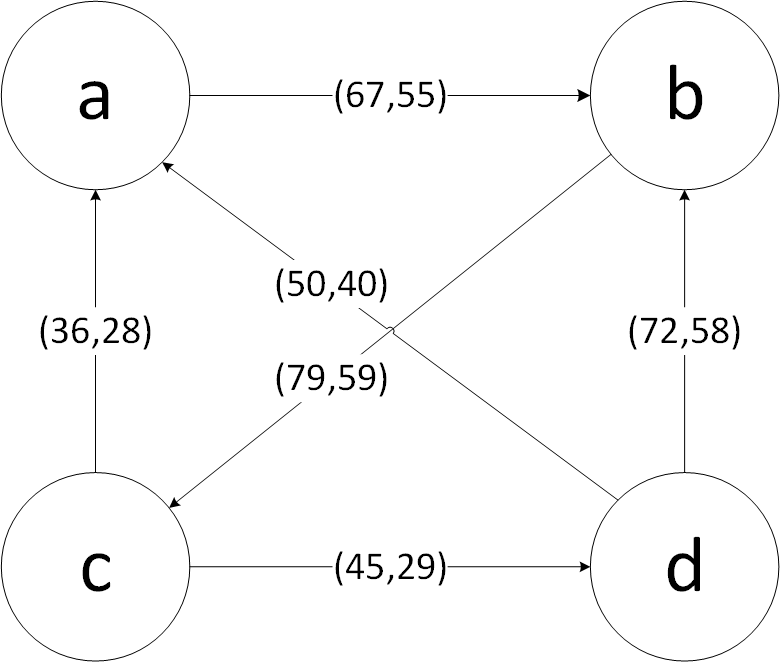
\includegraphics[scale=0.5]{Bilder/Beispiel3_Graph.png}
\caption{Graph über die Menge $N$(Beispiel 3)}
\label{fig:graph3}
\end{figure}

\subsection{Ergebnis} 
\label{sec:ergebnis3}

